\documentclass[11pt,a4paper]{article}
\usepackage[a4paper,margin=2.4cm]{geometry}
\usepackage[portuguese]{babel}
\usepackage{graphicx}
\usepackage{booktabs}
\usepackage{tabularx}
\usepackage{xcolor}
\usepackage{fancyhdr}
\usepackage{listings}
\usepackage{enumitem}
\usepackage{array}
\usepackage{amssymb}
\usepackage{hyperref}

\graphicspath{{prints/}}
\hypersetup{
  colorlinks=true,
  linkcolor=black!55!blue,
  urlcolor=black!55!blue,
  pdftitle={Implementacao 4 - Sincronizacao do Metro (ddc)},
  pdfauthor={ddc@cesar.school}
}

\pagestyle{fancy}
\raggedbottom
\fancyhf{}
\rhead{\small Implementação 4 -- Sincronização do Metrô}
\lhead{\small ddc}
\cfoot{\thepage}

\newcolumntype{L}[1]{>{\raggedright\arraybackslash}p{#1}}
\newcolumntype{Y}{>{\raggedright\arraybackslash}X}
\newcommand{\ok}{\textcolor{green!45!black}{\textbf{OK}}}
\setlength{\emergencystretch}{2em}

\lstset{
  basicstyle=\ttfamily\footnotesize,
  breaklines=true,
  columns=fullflexible,
  keepspaces=true,
  frame=single,
  backgroundcolor=\color{gray!12},
  framesep=3pt,
  xleftmargin=2mm
}

\begin{document}

\begin{center}
  {\LARGE\bfseries Implementação 4 -- Sincronização do Metrô}\\[6pt]
  {\large Relatório de atividade -- Infraestrutura de Software, CESAR School}\\[6pt]
  Daniel Donaire -- \texttt{ddc@cesar.school}\\
  Data: 4 de novembro de 2026
\end{center}
\vspace{4pt}

\section{Objetivo}

O enunciado pede a implementação em C da sincronização de uma estação de metrô:
a \texttt{struct station} e as quatro funções \texttt{station\_init},
\texttt{station\_load\_car}, \texttt{station\_wait\_for\_car} e
\texttt{station\_on\_board}, usando exclusivamente mutex e variáveis de condição
da POSIX \texttt{pthreads}: no máximo um lock por estação, sem semáforos, sem
espera ativa e com embarque simultâneo de vários passageiros em um mesmo carro.
Entregamos o código (\texttt{sync\_car.c}/\texttt{sync\_car.h}), o
\texttt{Makefile} que gera o executável \texttt{sync\_car}, o
\texttt{evidencias.log} da sessão de desenvolvimento, os dois prints obrigatórios
e este relatório; o runner \texttt{sync\_car-runner.c} foi fornecido pelo
professor e vai ser entregue sem nenhuma modificação.

\section{Checklist de Requisitos}

\noindent{\small
\noindent\begin{tabularx}{\textwidth}{L{6.2cm} c Y}
\toprule
\textbf{Requisito do enunciado} & \textbf{Status} & \textbf{Como testar / evidência} \\
\midrule
Implementar as quatro funções da API em C & \ok &
\texttt{./sync\_car} imprime \texttt{Looks good!} e retorna 0 (log 15:06). \\
\addlinespace
Usar apenas \texttt{pthreads} (mutex + variáveis de condição) & \ok &
\texttt{grep -n "pthread\_" sync\_car.c} lista só \texttt{mutex\_init/lock/unlock} e
\texttt{cond\_init/wait/signal/broadcast} (log 15:06). \\
\addlinespace
Nenhum semáforo ou outra primitiva & \ok &
\texttt{grep -ni "sem\_"} nos fontes retorna \texttt{semaphore: not found} (log 15:06). \\
\addlinespace
No máximo um lock por \texttt{station} & \ok &
\texttt{grep -c pthread\_mutex\_t sync\_car.h} $\rightarrow$ \texttt{1};
há apenas \texttt{pthread\_mutex\_t lock} na estrutura (log da sessão final). \\
\addlinespace
Sem busy-wait (espera ativa) & \ok &
Todo \texttt{while} de espera contém \texttt{pthread\_cond\_wait}; não há
\texttt{usleep}/\texttt{nanosleep}/\texttt{sched\_yield} nos fontes (grep vazio). \\
\addlinespace
Embarque simultâneo (vários passageiros no mesmo carro) & \ok &
Harness auxiliar fora do repositório: 10 threads passam por
\texttt{wait\_for\_car} antes do primeiro \texttt{on\_board} $\rightarrow$
\texttt{SIMULTANEIDADE OK} e \texttt{simul exit: 0} (log da sessão final). \\
\addlinespace
\texttt{count} = assentos livres: aceita 0, negativo e mais assentos que passageiros & \ok &
Caso limite/inválido: \texttt{station\_load\_car} com 0, $-5$ e 200 assentos
retorna sem travar $\rightarrow$ \texttt{LIMITE OK} (log da sessão final). \\
\addlinespace
\texttt{Makefile} gera o executável \texttt{sync\_car} & \ok &
\texttt{make} termina com \texttt{cc -o sync\_car sync\_car.o sync\_car-runner.o -pthread} (log 15:06). \\
\addlinespace
Runner do professor entregue sem modificação & \ok &
\texttt{sha256sum sync\_car-runner.c} confere a integridade do arquivo original (log da sessão final). \\
\addlinespace
\texttt{evidencias.log} com data, usuário, diretório e comandos reais & \ok &
Sessões \texttt{script(1)} de 14:34 a 22:59, cada uma iniciando com
\texttt{date; whoami; pwd; uname -a; gcc --version} (seção 6.1). \\
\addlinespace
Dois prints obrigatórios (erro principal + validação final) & \ok &
\texttt{prints/erro-early-return.png} e \texttt{prints/validacao-final.png} (seção 6.2). \\
\addlinespace
Relatório no formato do guia (seções 1--9) & \ok &
Este documento (\texttt{ddc.pdf}). \\
\bottomrule
\end{tabularx}
}

\section{Como Reproduzir}

Ambiente testado: Ubuntu 26.04 LTS em WSL2 (Windows~11), \texttt{gcc} 15.2.0,
GNU Make 4.4.1. O programa não recebe argumentos nem entrada do usuário.

\begin{lstlisting}
make clean
make
./sync_car
\end{lstlisting}

Saída esperada (trecho): linhas \texttt{car entering station with N free seats}
/\texttt{car departed station with N new passenger(s) (expected N)} e, ao final:

\begin{lstlisting}
Looks good!
\end{lstlisting}

Para confirmar o código de saída:

\begin{lstlisting}
echo $?
# 0
\end{lstlisting}

O runner também pode ser chamado por \texttt{make test}. A compilação com
avisos estritos (\texttt{-Wextra -Werror}) é feita por \texttt{make check}.

\section{Arquitetura (resumida)}

\textbf{Arquivos e responsabilidades:}

\noindent\begin{tabularx}{\textwidth}{L{5.2cm} Y}
\toprule
\textbf{Arquivo} & \textbf{Responsabilidade} \\
\midrule
\texttt{sync\_car.c} & Implementação das quatro funções da estação. \\
\texttt{sync\_car.h} & \texttt{struct station} (1 mutex, 2 variáveis de condição, 4 contadores) e protótipos. \\
\texttt{sync\_car-runner.c} & Programa principal de teste do professor (não modificado). \\
\texttt{Makefile} & Alvos \texttt{all}, \texttt{check}, \texttt{test} e \texttt{clean}. \\
\texttt{evidencias.log} & Sessão \texttt{script(1)} com comandos, saídas, data, usuário e diretório. \\
\texttt{prints/} & Print do erro principal e da validação final. \\
\bottomrule
\end{tabularx}

\vspace{6pt}
\textbf{Decisões técnicas:}

\noindent\begin{tabularx}{\textwidth}{L{5.6cm} L{5.4cm} Y}
\toprule
\textbf{Decisão} & \textbf{Motivo} & \textbf{Consequência} \\
\midrule
\texttt{count} tratado como assentos livres e clampado
(\texttt{count > 0 ? count : 0}) &
O enunciado define \texttt{count} como assentos livres do carro; valores
inválidos não podem travar o processo &
\texttt{load\_car(0)} e \texttt{load\_car($-5$)} retornam imediatamente e o caso
``mais assentos que passageiros'' converge sozinho quando \texttt{waiting} chega a 0. \\
\addlinespace
Contador \texttt{boarding} + variável de condição \texttt{passenger\_boarded}
(estratégia S2) &
S1 não esperava o embarque e o runner abortava com
\texttt{station\_load\_car returned early!} &
O carro só parte depois de concluído o embarque dos passageiros admitidos
(ou quando não há ninguém esperando e ainda sobram assentos); assim a saída do
carro passa a ser observável pelo runner. \\
\addlinespace
Uma variável de condição por direção: \texttt{car\_arrived}
(passageiros) e \texttt{passenger\_boarded} (carro) &
Com um único lock, duas direções de espera precisam ser sinalizadas
separadamente &
\texttt{pthread\_\allowbreak cond\_\allowbreak broadcast} acorda todos os passageiros quando o carro
chega; \texttt{pthread\_cond\_signal} devolve o controle ao carro após cada
embarque, sem \emph{lost wakeup}. \\
\addlinespace
Condição de saída do carro:
\texttt{boarding > 0 || (free\_seats > 0 \&\& waiting > 0)} &
O runner exige que \texttt{load\_car} não retorne antes de
\texttt{MIN(passengers\_left, free\_seats)} embarcarem, nem depois de o embarque
terminar &
O carro bloqueia enquanto há embarque em andamento ou assento para quem espera,
e retorna no máximo ~1\,s após o último \texttt{on\_board} (janela de espera do
runner). \\
\bottomrule
\end{tabularx}

\section{Estratégias e Diário de Desenvolvimento}

\subsection{Estratégias da semana}

\noindent\begin{tabularx}{\textwidth}{c L{3.4cm} Y Y}
\toprule
 & \textbf{Nome curto} & \textbf{Contexto} & \textbf{Motivo da troca (se houve)} \\
\midrule
S1 & Carro publica assentos &
Primeira implementação: \texttt{station\_load\_car} define
\texttt{car\_present}/\texttt{free\_seats}, faz \texttt{broadcast} e \texttt{return}; \texttt{on\_board} era vazio &
-- \\
S2 & Contador de embarque &
Correção após a falha do runner: adiciona \texttt{boarding},
\texttt{passenger\_boarded} e o laço de espera na saída do carro &
S1 fazia \texttt{load\_car} retornar imediatamente (o runner chamava
\texttt{load\_car} antes de os passageiros embarcarem) $\rightarrow$
\texttt{Error: station\_load\_car returned early!} \\
S3 & (não utilizada) & -- & -- \\
\bottomrule
\end{tabularx}

\subsection{Diário de Tentativas}

\noindent{\footnotesize\setlength{\tabcolsep}{2.85pt}
\noindent\begin{tabularx}{\dimexpr\textwidth-3pt\relax}{c c Y Y Y c Y}
\toprule
\# & \textbf{Estrat.} & \textbf{O que tentei} & \textbf{Resultado} &
\textbf{Hipótese\allowbreak/Causa (se falhou)} & \textbf{Quando} & \textbf{Evidência} \\
\midrule
1 & S1 & Abertura da sessão de evidências (\texttt{script -a evidencias.log})
e identificação do ambiente (\texttt{date}, \texttt{whoami}, \texttt{pwd},
\texttt{uname -a}, \texttt{gcc --version}) &
Log iniciado; terminal reaberto em seguida (duas sessões curtas de
\texttt{exit}) & -- & 14:34--14:35 & \texttt{evidencias.log}, blocos 1--3 \\
\addlinespace
2 & S1 & \texttt{make clean}, \texttt{make}, \texttt{make check} e primeira
execução do \texttt{./sync\_car} &
\textbf{Falha:} \texttt{Error: station\_\allowbreak load\_\allowbreak car returned early!},
\texttt{exit code: 1} &
\texttt{station\_\allowbreak load\_\allowbreak car} só publicava os assentos e retornava sem esperar o
embarque; o runner detectou a saída prematura do carro &
14:38--14:39 & \texttt{evidencias.log}, bloco 14:38:53; print
\texttt{erro-early-\allowbreak return.png} \\
\addlinespace
3 & S2 & Reescrita com o contador \texttt{boarding} e a variável de condição
\texttt{passenger\_\allowbreak boarded}; \texttt{make clean}, \texttt{make},
\texttt{make check}, \texttt{./sync\_car} &
\texttt{Looks good!} e \texttt{exit code: 0} & -- & 15:06 &
\texttt{evidencias.log}, bloco 15:06:02--15:06:58 \\
\addlinespace
4 & S2 & Auditoria dos requisitos por \texttt{grep} (campos da estrutura,
funções \texttt{pthread}, busca por semáforo) &
Estrutura com 1 mutex e 2 variáveis de condição; \texttt{semaphore: not found} & -- & 15:06 & Mesmo bloco \\
\addlinespace
5 & S2 & 100 execuções seguidas do runner (\texttt{for i in 1..100}) &
\texttt{100 iteracoes OK} (duas tentativas anteriores canceladas com
\texttt{\^C} antes de completar) & -- & 16:14 &
\texttt{evidencias.log}, bloco 16:13:59--16:15:55 \\
\addlinespace
6 & S2 & Harness de simultaneidade em \texttt{/tmp/simul.c}: 10 passageiros
esperam antes do primeiro \texttt{on\_board} &
\texttt{SIMULTANEIDADE OK} e \texttt{simul exit: 0} & -- & 22:58 &
\texttt{evidencias.log}, sessão 22:58--22:59 \\
\addlinespace
7 & S2 & Caso limite/inválido (\texttt{count} = 0, $-5$ e 200), integridade do
runner (\texttt{sha256sum}), contagem de locks e listagem dos prints &
\texttt{LIMITE OK}, runner íntegro, \texttt{grep -c} $= 1$, \texttt{Looks good!}
no print & -- & 22:58 & \texttt{evidencias.log}, sessão 22:58--22:59;
\texttt{prints/} \\
\bottomrule
\end{tabularx}
}

\section{Evidências}

\subsection{Log automático}

No início de cada sessão de trabalho foi executado
\texttt{script -a evidencias.log}, que grava automaticamente todos os comandos
e saídas do terminal. Toda sessão começa com \texttt{date}, \texttt{whoami},
\texttt{pwd}, \texttt{uname -a} e \texttt{gcc --version}, de modo que o log
carrega sozinho data, usuário, diretório e ferramentas. O arquivo
\texttt{evidencias.log} (enviado dentro do \texttt{.tar}) contém 7 sessões
entre 14:34 e 22:59 de 04/11/2026, incluindo a falha da estratégia S1, a
correção S2, a auditoria de requisitos, o teste de 100 execuções e a sessão
final (22:58--22:59), com o caso limite/inválido, a integridade do runner
(\texttt{sha256sum}), a contagem de locks e o teste de simultaneidade.

\subsection{Prints}

\textbf{Erro principal:} o momento do bug mais relevante da semana -- o runner
abortando porque \texttt{station\_load\_car} retornou antes do embarque
(estratégia S1):

\begin{center}
  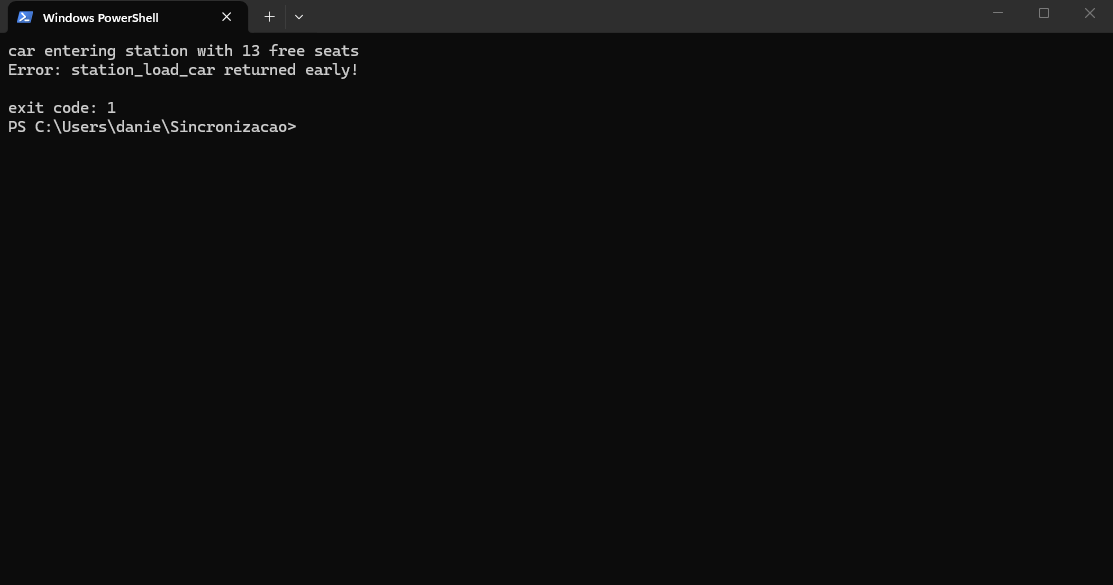
\includegraphics[width=0.92\textwidth]{erro-early-return.png}
\end{center}

\textbf{Validação final:} compilação do zero e execução do runner terminando em
\texttt{Looks good!}:

\begin{center}
  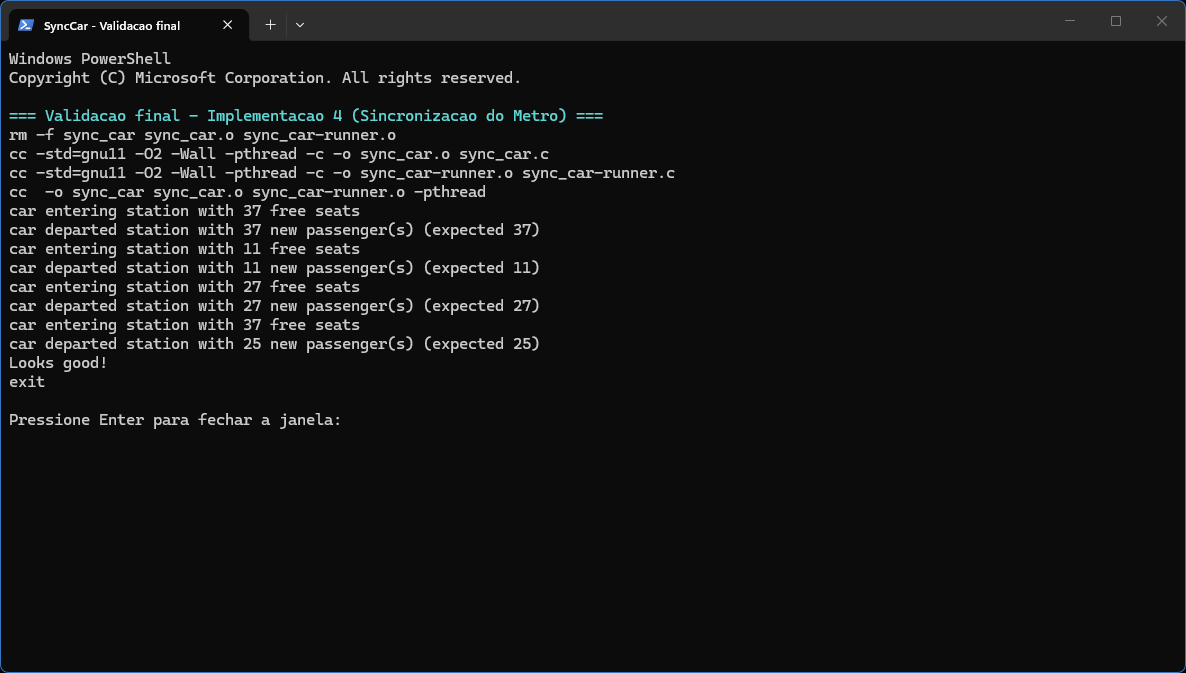
\includegraphics[width=0.92\textwidth]{validacao-final.png}
\end{center}

\section{Uso de IA}

\textbf{Onde usei IA (2--3 linhas):} utilizei um assistente de IA (OpenCode,
com modelo de linguagem) durante toda a atividade: leitura e decomposição das
restrições do enunciado e do guia de relatórios, discussão do desenho da
sincronização, rascunhos de código e de testes auxiliares fora do repositório,
auditoria dos requisitos por \texttt{grep} e montagem da estrutura deste
relatório.

\textbf{O que validei manualmente e como:} compilei e executei tudo no meu
terminal (\texttt{make}, \texttt{make check}, \texttt{./sync\_car}, 100
execuções seguidas, caso limite/inválido e harness de simultaneidade); conferi
pessoalmente cada \texttt{grep} de auditoria; revi linha a linha o código
entregue e este relatório antes de gerar o \texttt{ddc.pdf}; decidi sozinho
quando trocar de estratégia.

\section{Reflexão Final}

A principal lição da semana foi confiar no contrato do teste antes de codar:
S1 parecia correta, mas esquecia que \texttt{station\_load\_car} é uma operação
\emph{síncrona} do
carro: ela só pode retornar quando o embarque terminou. Isso causou o bug que
mais me travou (\texttt{returned early!}) e só foi resolvido quando passei a
ler o runner linha a linha e a modelar explicitamente quem espera por quem. A
decisão técnica mais importante foi adicionar o contador \texttt{boarding}:
sem ele, ``assentos esgotados'' e ``embarque em andamento'' eram indistinguíveis
na condição de saída. Também aprendi a separar as duas direções de espera em
variáveis de condição diferentes, o que eliminou a possibilidade de
\emph{lost wakeup} sem aumentar o número de locks. Em uma próxima atividade eu
faria os testes de concorrência (100 execuções e harness) logo na primeira
sessão, em vez de depois da correção, e manteria comentários no código desde o
início para reduzir o retrabalho de revisão.

\section{Checklist Final de Entrega}

\noindent\begin{tabularx}{\textwidth}{Y c}
\toprule
\textbf{Item} & \textbf{Confirmado?} \\
\midrule
Compilei do zero seguindo só o que está no relatório & $\checkmark$ \\
Rodei os testes e \texttt{evidencias.log} foi gerado & $\checkmark$ \\
Tenho prints obrigatórios & $\checkmark$ \\
Testei pelo menos um caso limite e um caso inválido & $\checkmark$ \\
Preenchi a seção de uso de IA & $\checkmark$ \\
Revisei o relatório e removi frases genéricas / vazias & $\checkmark$ \\
\bottomrule
\end{tabularx}

\end{document}



